\section{Finance Ontology}\label{sec:result_f_ontology}
In this section, results from the crowd-sourced ontology validation in the domain of finance are presented. A detailed discussion of the ontology used as a baseline for all calculations was done previously in \hyperref[sec:evaluation_datasets]{Section~\ref*{sec:evaluation_datasets}}.

As with the other datasets the~\emph{Metadata based Approach} performed quite well. In fact, it outperformed all other approaches, both in terms of Precision and Recall, yielding the highest value of F-Measure. A detailed comparison of all methods for this dataset is given in~\hyperref[table:bench_p_r_f_finance]{Table~\ref*{table:bench_p_r_f_finance}}. On the other end of the table is ontology validation without any Context enrichment~(\emph{None}). This is in line with our initial hypothesis that motivated the use of concept descriptions. We also noticed the relatively high number of Recall for all approaches. The same observation was made for the other datasets as well. Indeed, crowd workers tend to decline concepts in case of uncertainty or lack of additional information.
\begingroup
\renewcommand{\arraystretch}{1.5}
\begin{table}
	\begin{tabularx}{\textwidth}{l c*{3}{Y}}
		\toprule
		Method & Precision & Recall & F-Measure \\
		\midrule
		 Metadata based Approach & 0.797 & 0.985 & 0.881 \\
		 Dictionary based Approach & 0.794 & 0.944 & 0.862 \\
		 Ontology based Approach & 0.756 & 0.949 & 0.842 \\
		 None & 0.734 & 0.963 & 0.833 \\
		\bottomrule
	\end{tabularx}
	\caption{Aggregated results on the Finance Ontology~(ranked by F-Measure)}
	\label{table:bench_p_r_f_finance}
\end{table}
\endgroup

Another metric we used to measure the performance of ontology validation was Inter-rater agreement. 
\hyperref[fig:hist_agreement_finance_all]{Figure~\ref*{fig:hist_agreement_finance_all}} depicts the distribution of the agreement ratio among all validated concepts. For comparability, all methods were merged into one chart and grouped by the level of agreement. Again, the~\emph{Metadata based Approach} performed best followed by the~\emph{Ontology~based~Approach} as indicated by the red bar. It shows both, a high level of full agreement~($1$) and low level of little agreement~($0.6$). 
\begin{sidewaysfigure}
  	 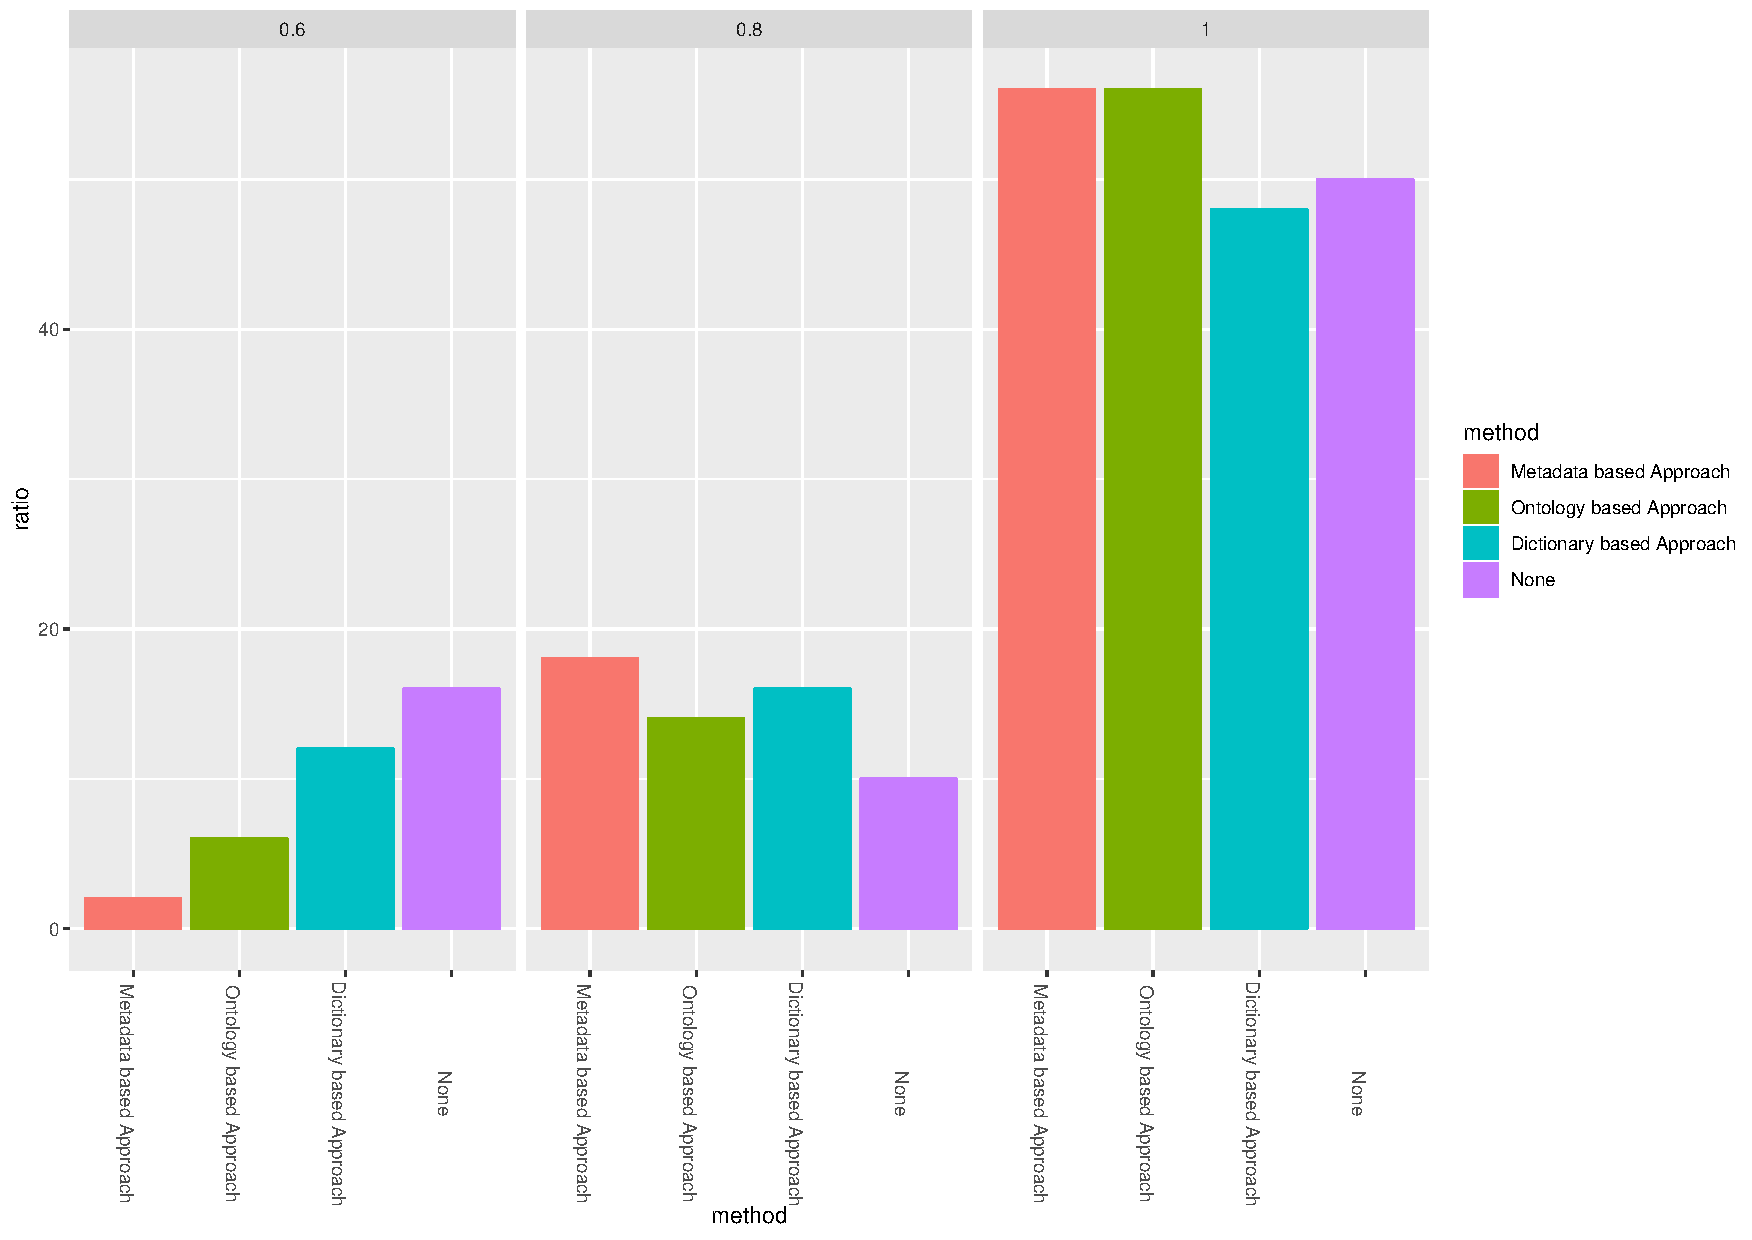
\includegraphics[width=\textwidth]{plots/finance/hist_agreement_corrected}
  	 \caption{Histogram plots of the Inter-rater Agreement}\label{fig:hist_agreement_finance_all}
\end{sidewaysfigure}
 
\begin{figure}
    \centering
    \begin{subfigure}[b]{0.4\textwidth}
        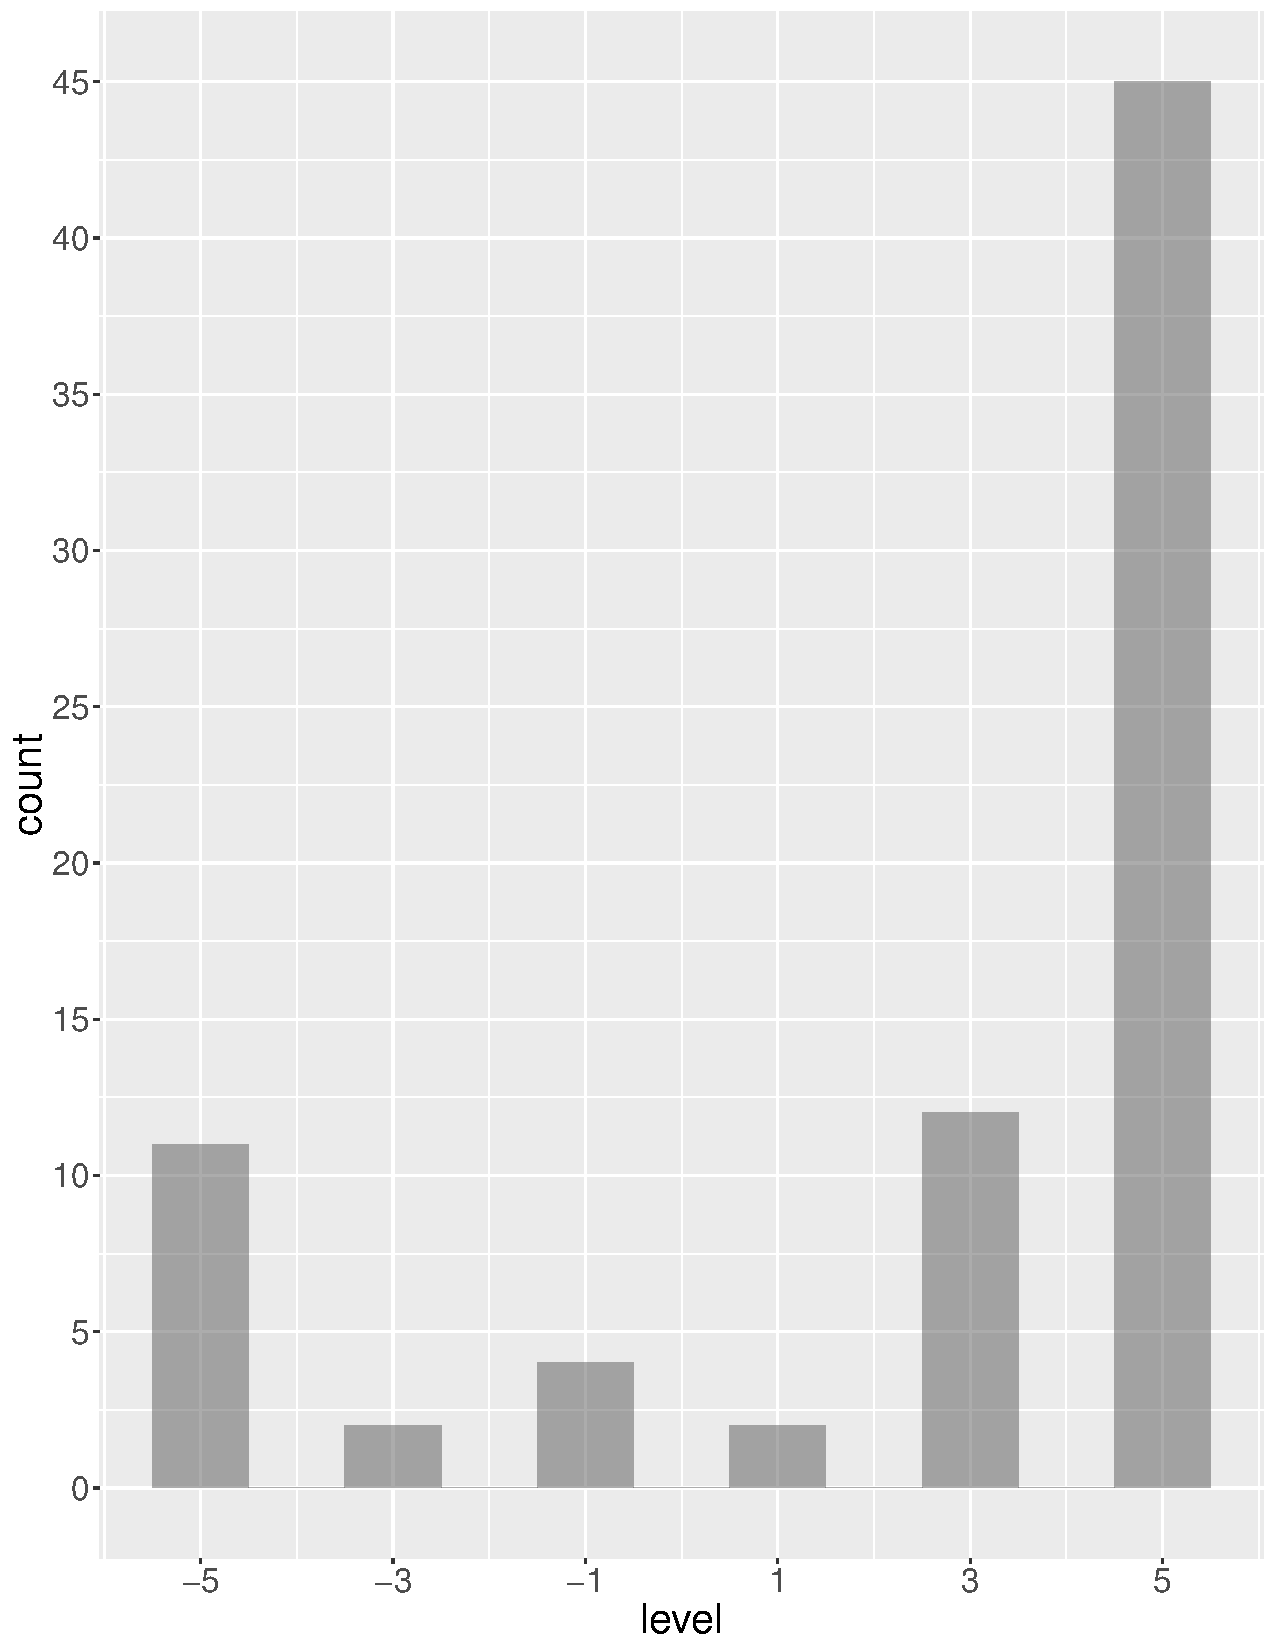
\includegraphics[width=\textwidth]{plots/finance/hist_level_nn}
        \caption{Ontology based Approach}
        \label{fig:hist_level_finance_nn}
    \end{subfigure}
    ~
    \begin{subfigure}[b]{0.4\textwidth}
        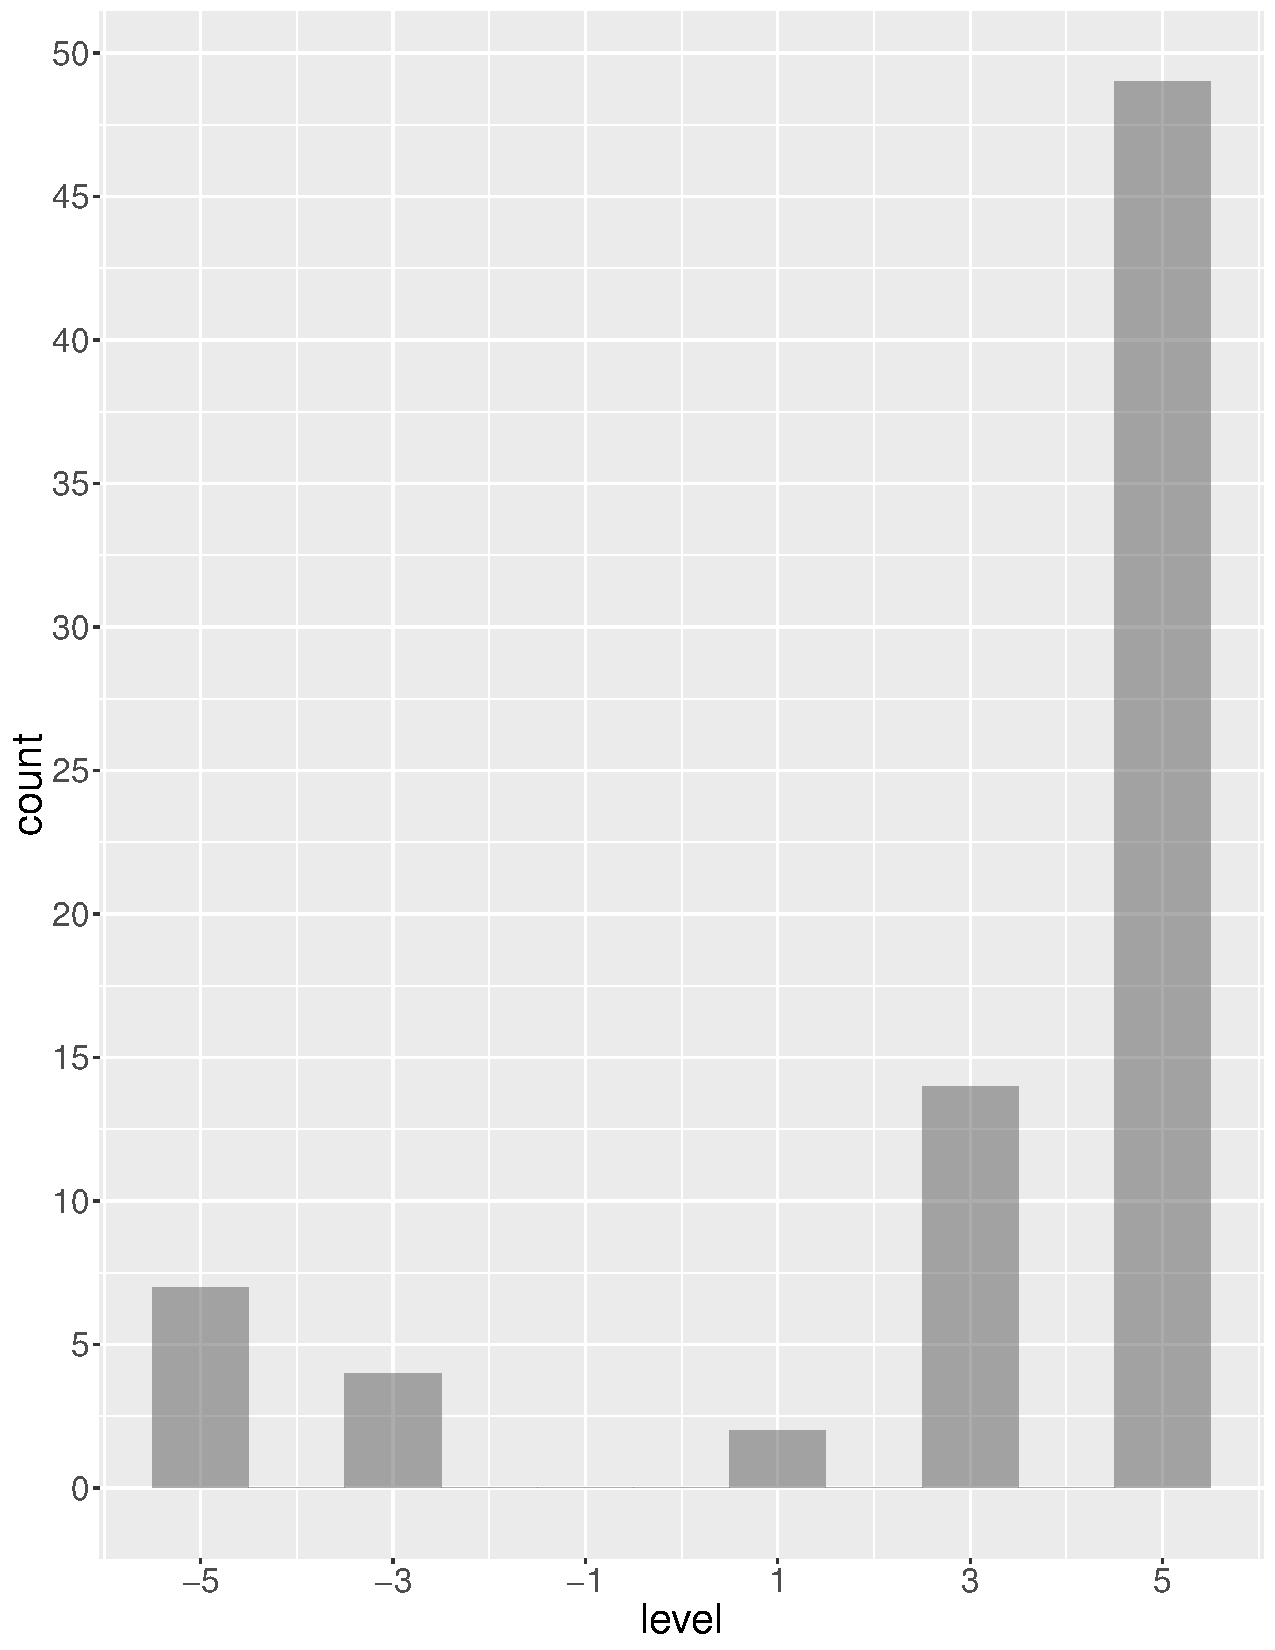
\includegraphics[width=\textwidth]{plots/finance/hist_level_ec}
        \caption{Metadata based Approach}
        \label{fig:hist_level_finance_ec}
    \end{subfigure}
    ~
    \begin{subfigure}[b]{0.4\textwidth}
        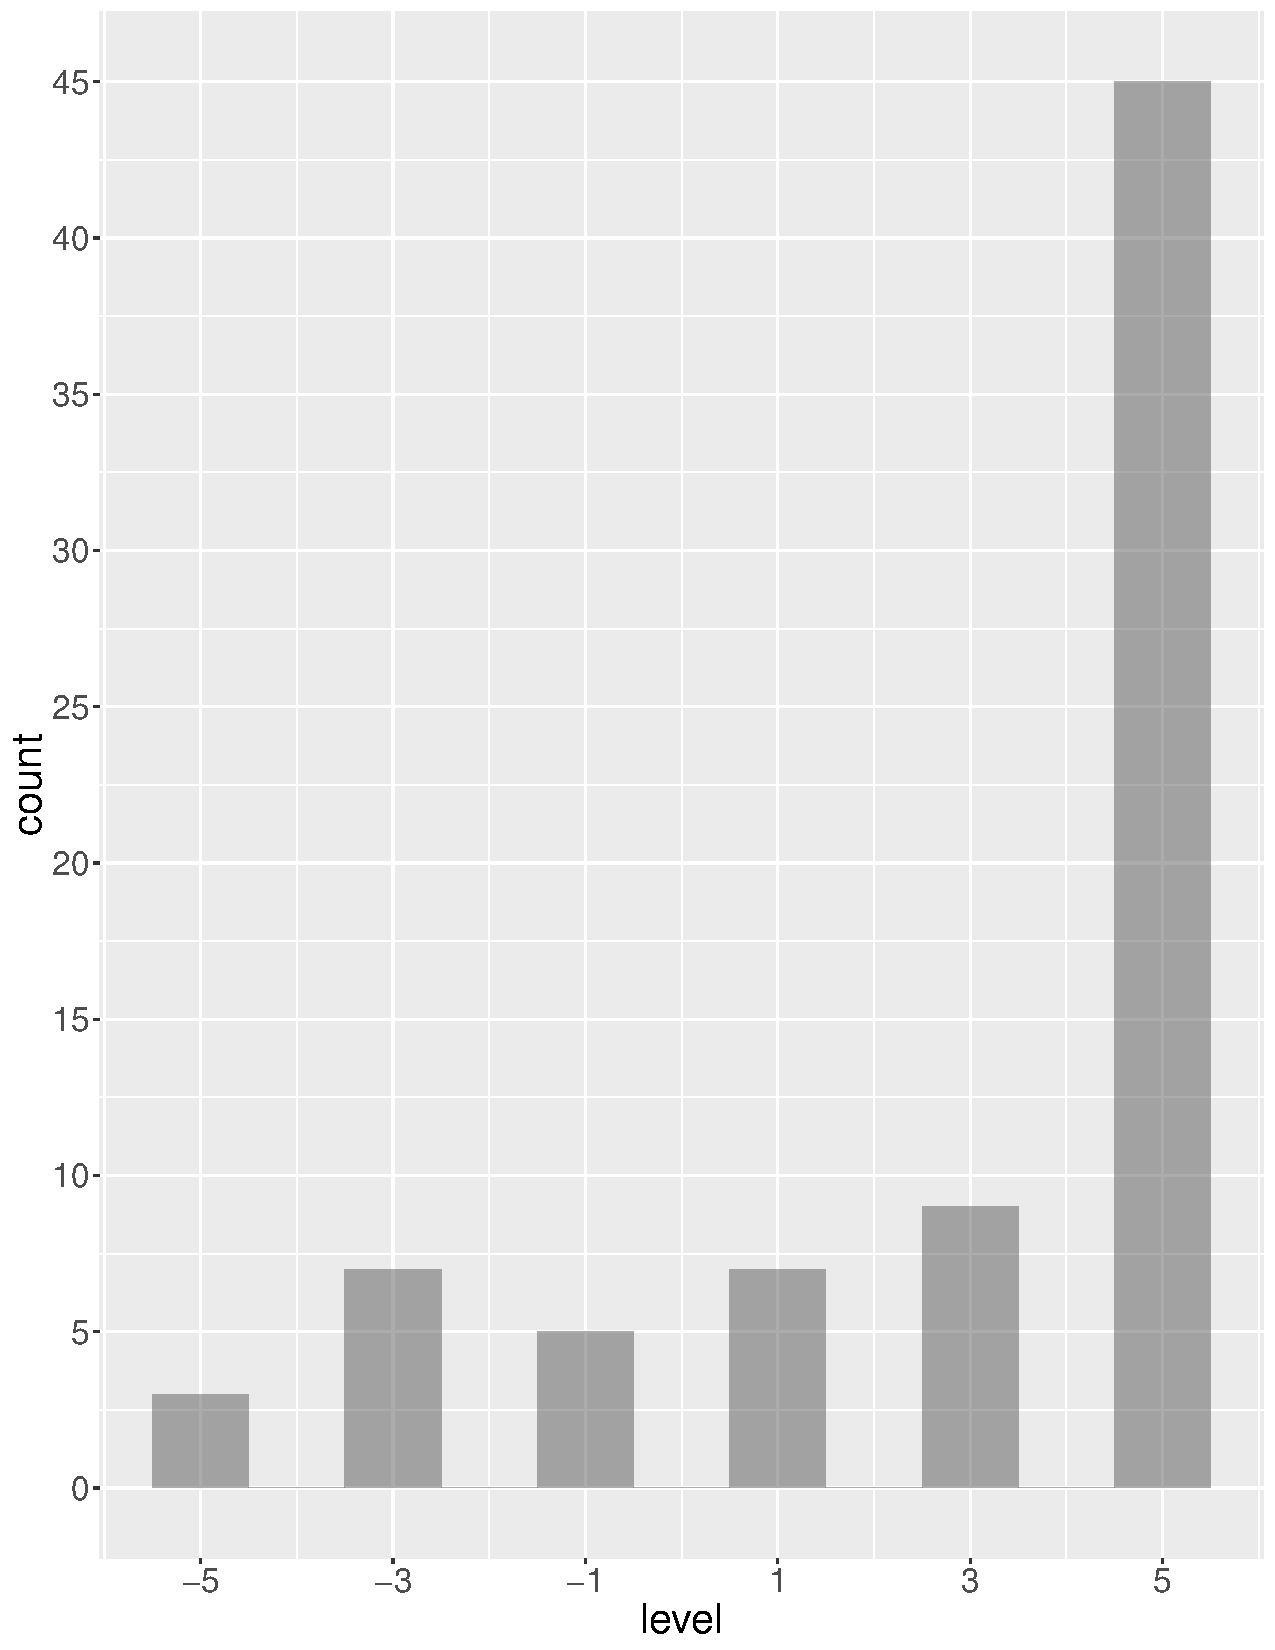
\includegraphics[width=\textwidth]{plots/finance/hist_level_es}
        \caption{Dictionary based Approach}
        \label{fig:hist_level_finance_es}
    \end{subfigure}
    ~
    \begin{subfigure}[b]{0.4\textwidth}
        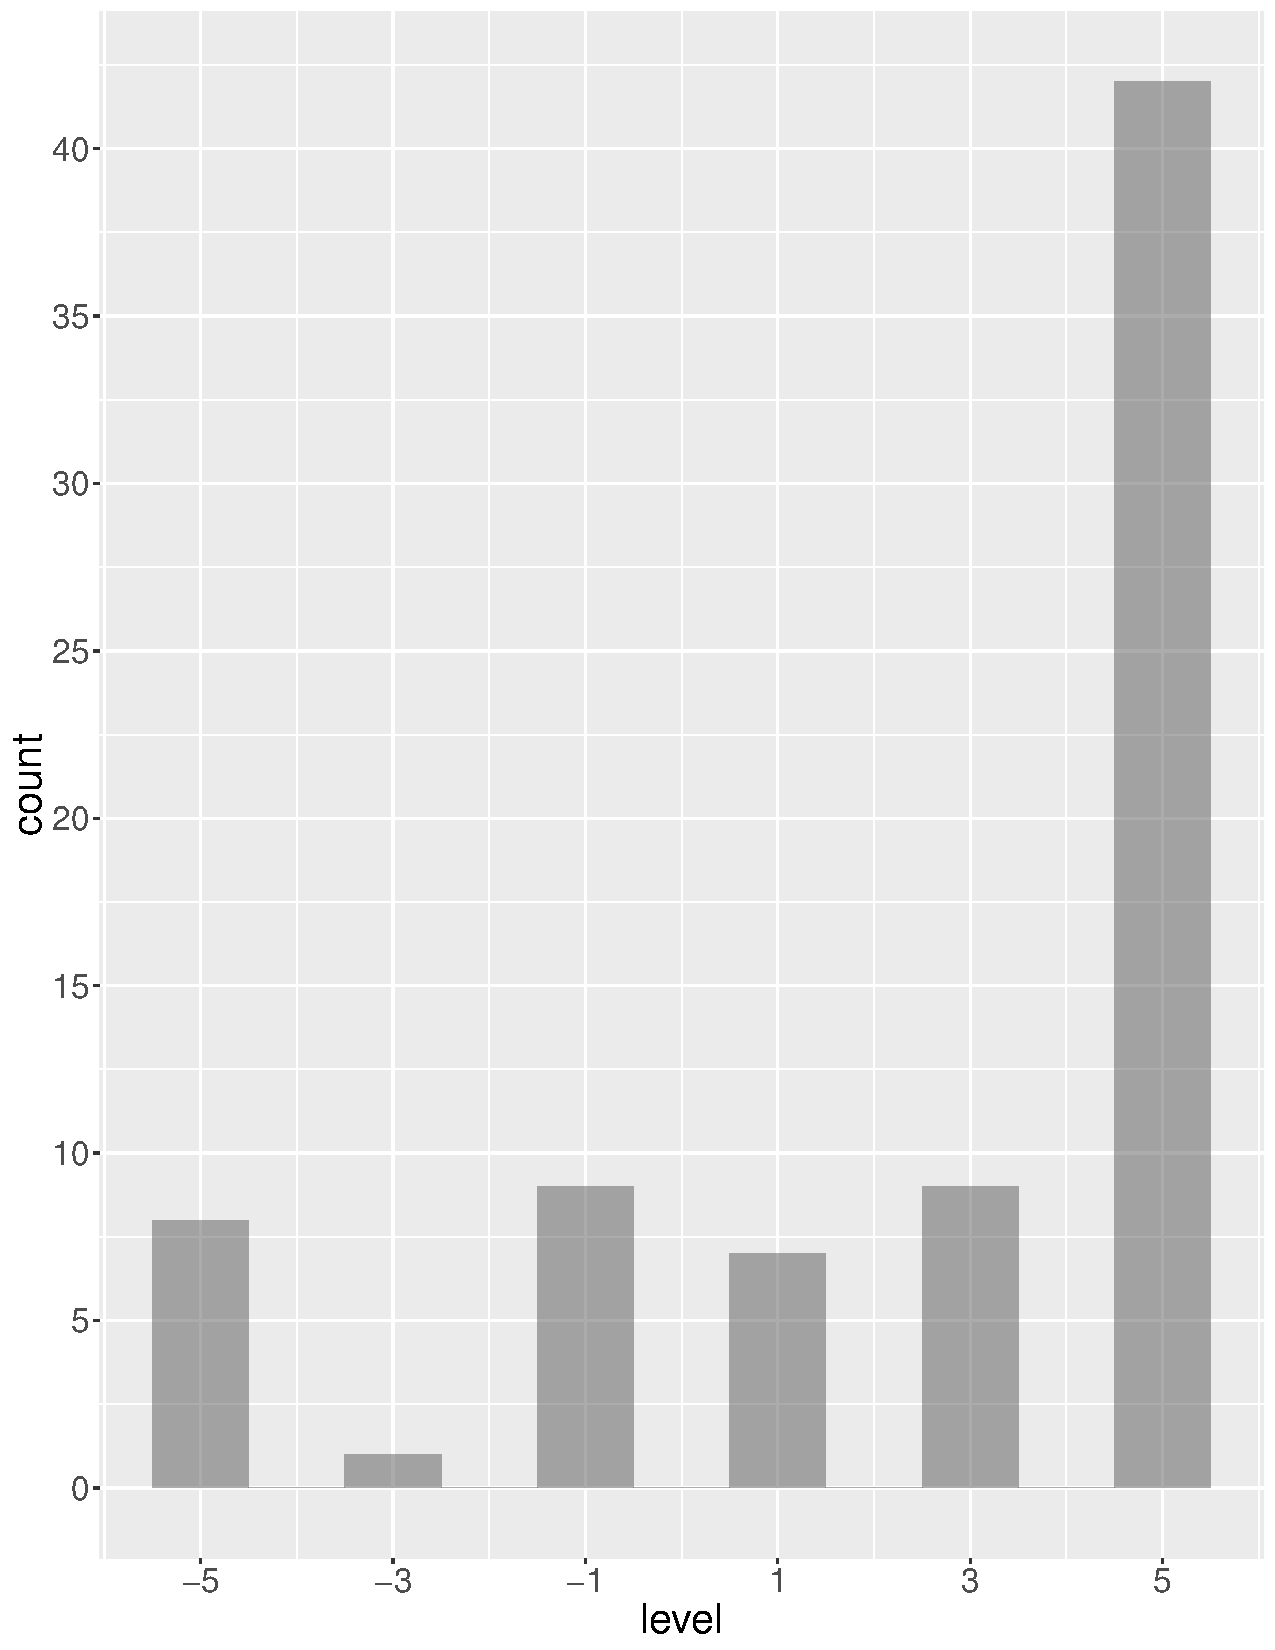
\includegraphics[width=\textwidth]{plots/finance/hist_level_none}
        \caption{None}
        \label{fig:hist_level_finance_none}
    \end{subfigure}
	\caption{Histogram plots of the correct/incorrect judgements. $\{$\emph{count}=number of judgements, \emph{level}=combined number of correct (positive scale) and incorrect (negative scale) judgements per concept$\}$ }
	\label{fig:hist_level_finance_all}
\end{figure}

To get a different view of the overall worker performance, \hyperref[fig:hist_level_finance_all]{Figure~\ref*{fig:hist_level_finance_all}} 
shows bar plots of the performance levels. Each level combines the agreement ratio with the amount of correct/incorrect judgements, yielding a higher score when most contributors agreed on correct answers and a lower score when they disagreed or answered incorrectly.
A common phenomena of all approaches was the high level of correct answers with high agreement across contributors. Indeed, this holds for the other datasets too. However, after analysing the concepts that were accepted and those that were declined, this is rather related to the generic nature of the used datasets. For example, whereas accepting the concept \emph{budget} for the finance domain is relatively easy even with no additional information, judging the concept \emph{world} is much more challenging. Therefore, judging generic concepts should be done better by domain experts who share a common understanding of the used vocabulary. 

\begingroup
\renewcommand{\arraystretch}{1.5}
\begin{table}
	\begin{tabularx}{\textwidth}{l c*{4}{Y}}
		\toprule
		Method & mean & median & $1^{st}$ quartile & $3^{rd}$ quartile \\
		\midrule
		 Metadata based Approach & 3.18 & 5.00 & 3.00 & 5.00 \\
		 Dictionary based Approach & 2.87 & 5.00 & 1.00 & 5.00 \\
		 Ontology based Approach & 2.61 & 5.00 & 2.50 & 5.00 \\
		 None & 2.53 & 5.00 & 1.00 & 5.00 \\
		\bottomrule
	\end{tabularx}
	\caption{Summary statistics concerning agreement level on the Finance Ontology~(ranked by mean value)}
	\label{table:level_corr_incorr_finance}
\end{table}
\endgroup

The summary statistics in~\hyperref[table:level_corr_incorr_finance]{Table~\ref*{table:level_corr_incorr_finance}} confirm our observations made so far. It shows the statistics of each method ranked by mean value. Judging the worker performance by the level of agreement and the ratio of correct/incorrect judgements, the order is no different than ranked by F-Measure. 
